\chapter{Conceptional System Design}


\section{MVC Pattern}
\label{mvc}

The Model-View-Controller (MVC) is a software architecture pattern for user interface implementation, where the application logic is separated from the user interface.

In object-oriented programming the Model is the objects where the data from the database is stored. The View is the presentation layer, what the user sees and interacts with. The Controller will process and respond to the user requests and invoke the changes in the Model. 

The MVC pattern is memory efficient, because multiple views can share the same underlying data model. Controllers can be separated by events. This let's the developer to create a controller hierarchy, because a controller for a keyboard event is different from a controller for a mouse event. Views implement an instance of a controller, that can be changed at run-time, because we can be disabled and enabled.


\begin{figure}[!ht]
	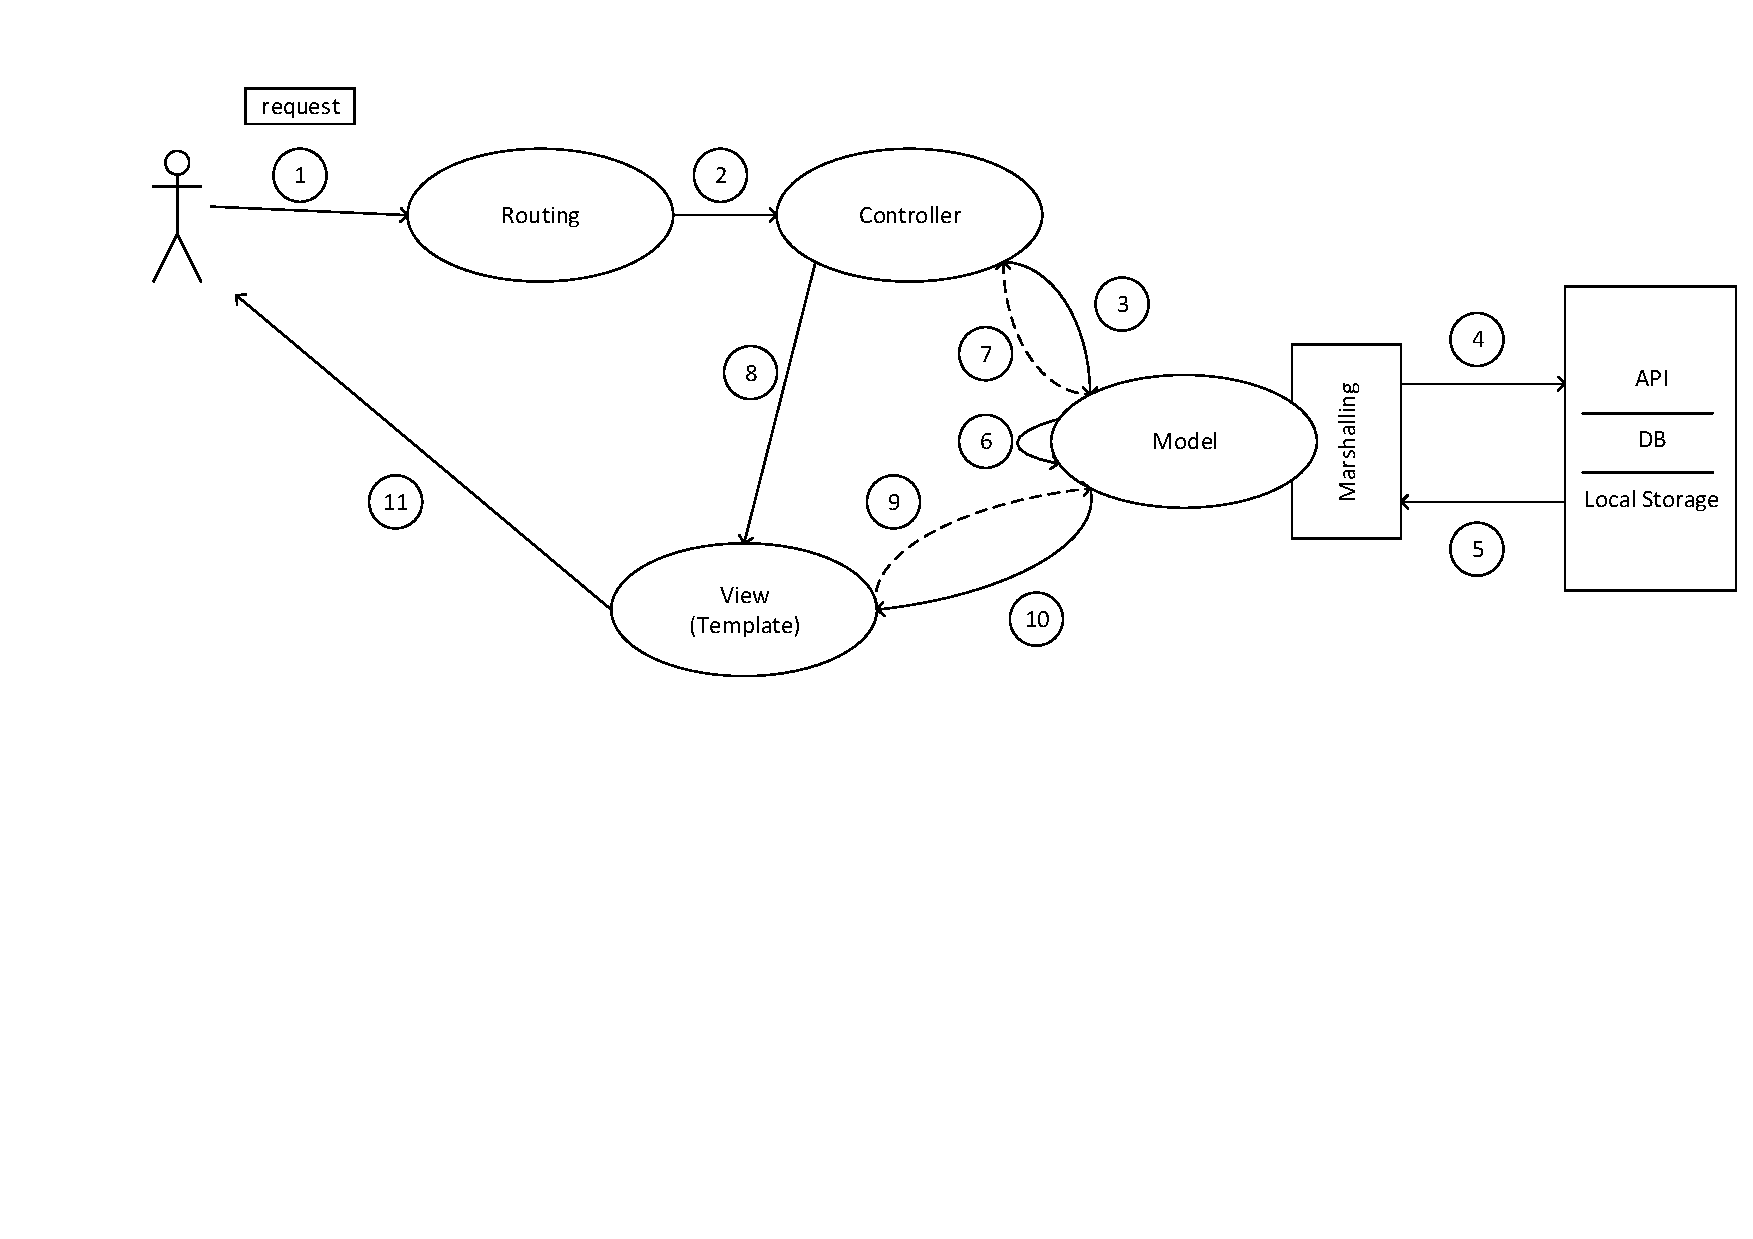
\includegraphics[width=\textwidth]{figures/klasszikus_mvc_webalkalmazas.pdf}
	\caption{Classic MVC Webapplication \\ Made by Bence Golda}
	\label{fig:classic-mvc-webapplication}
\end{figure}

In webapplications the browser communicates with a controller. When the user sends a request, routing will decide which controller will handle the request. The chosen controller talks to the model to get the relevant data. If it's necessary, the model will send data to or ask for data from the database, the API or the local storage. During this process, the data has to be transformed via marshalling. Marshalling is the process, that transforms the data between storable and sendable dataformats. When the model returns the desired data to the controller, it will forward the data to the view. The presentation layer will decide which page has to be returned to the browser, binds the data to the view template and returns it.

\section{System Design}

\begin{figure}[!ht]
	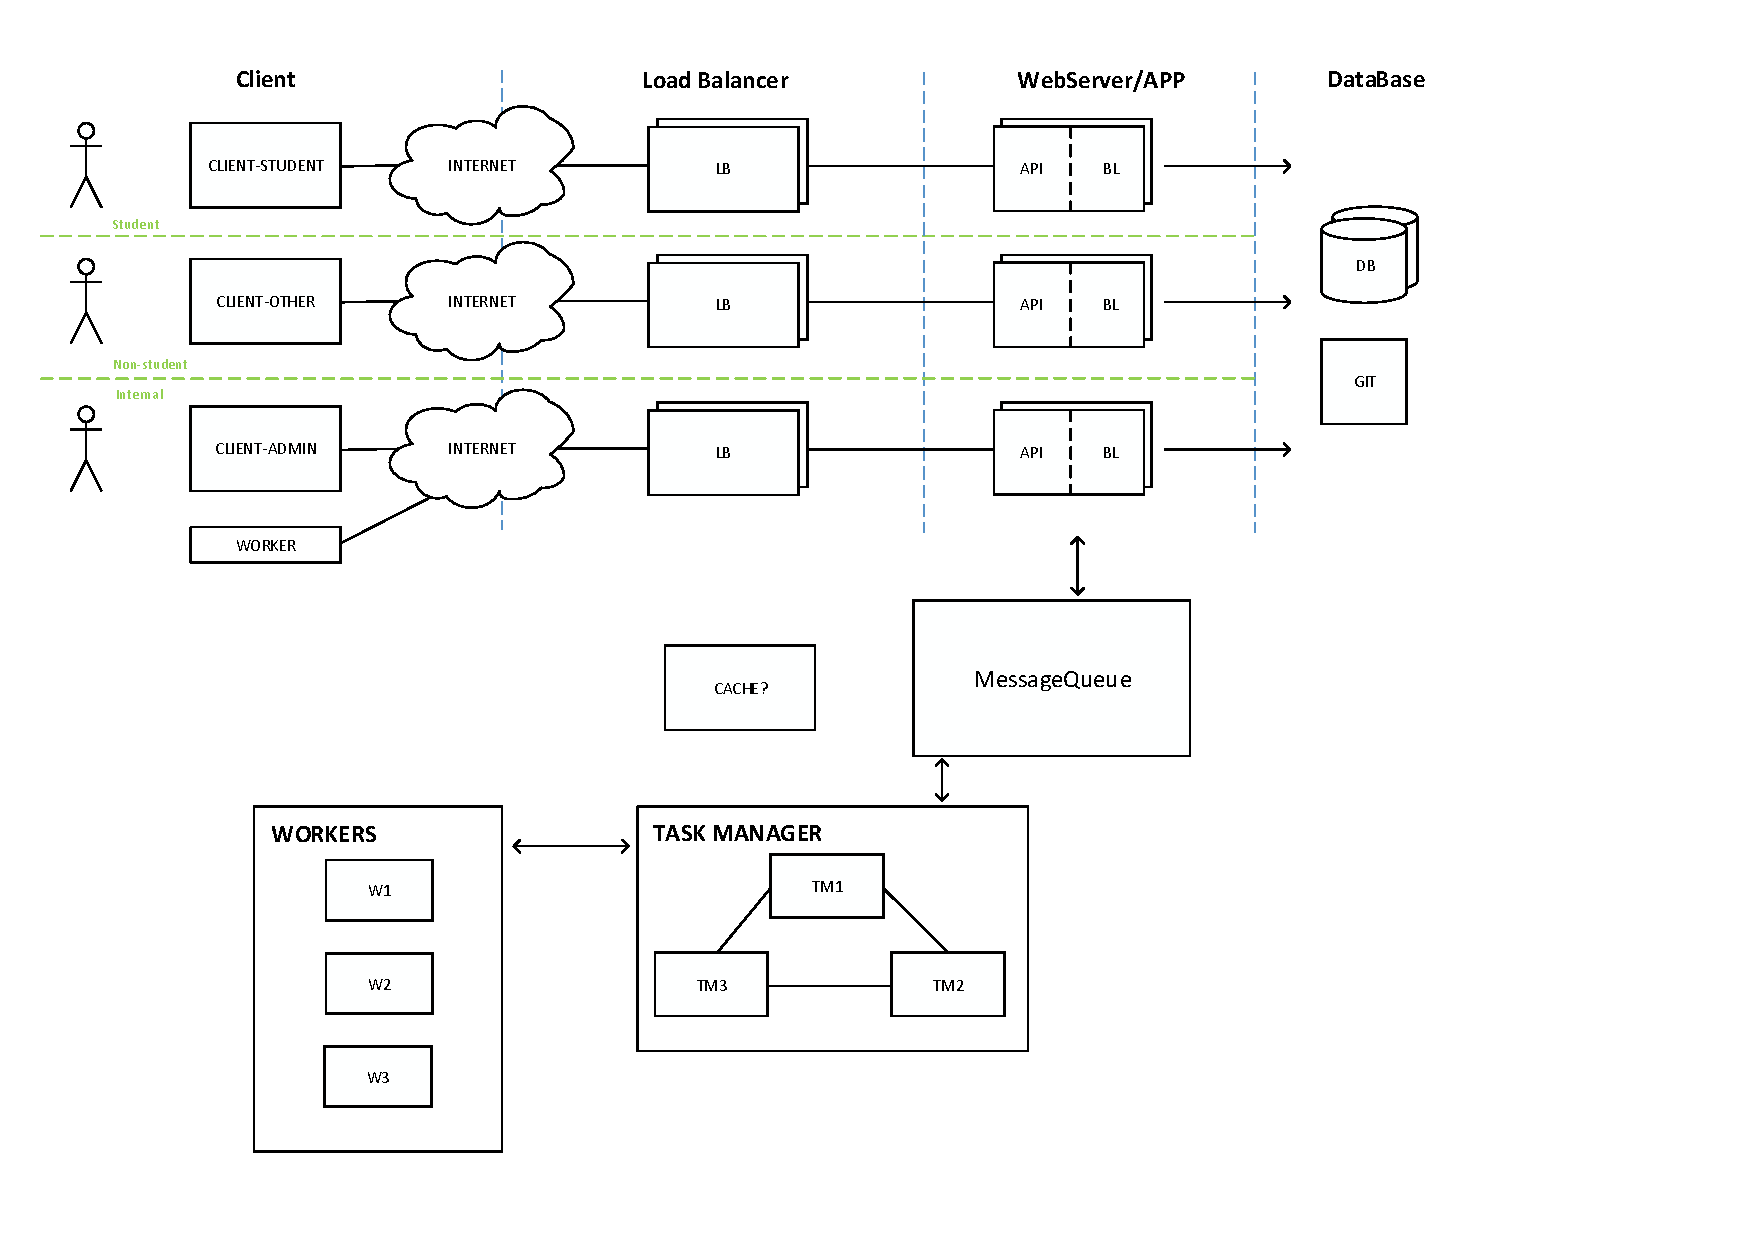
\includegraphics[width=\textwidth]{figures/atfogo_rendszerterv.pdf}
	\caption{Conceptional System Design}
	\label{fig:conceptional-system-design}
\end{figure}

\todo{ábramagyarázat}

\subsection{Frontend System Design}
\todo{frontend ábra}

\subsection{Database - ER}

\subsection{Server}

\subsection{client-server commmunication}

\subsection{client-user commmunication}